Tools were run on the function \texttt{send\_publish\_notifications(..)} and on the file \texttt{tools.py}.

\paragraph{Pylint}
The Python quality checker \emph{Pylint} is a tool to help with coding standard as recommended by PEP 8, error detection and refactoring.
Pylint message categories:
\begin{itemize}
    \item (C) convention: programming standard violation
    \item (R) refactor: code smell
    \item (W) warning: python specific problem
    \item (E) error: likely bug
    \item (F) fatal: an error occurred preventing pylint from continuing the analysis
\end{itemize}
\begin{figure}[h]
    \centering
    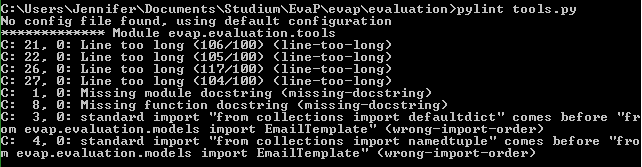
\includegraphics[width=\textwidth, keepaspectratio]{graphics/pylint_send_publish_notifications_1}
    \caption{Pylint messages for \texttt{send\_publish\_notifications(..)}}
    \label{fig:pylint}
\end{figure} 
As expected after our testing Pylint found mostly violated coding conventions in \texttt{send\_publish\_notifications(..)} (\ref{fig:pylint}). 
The investigation of the file \texttt{tools.py} leads to a few warnings and refactoring hints that we will discuss with the developers on the next occasion.
%TODO Restliche Grafiken in den Anhang?


\paragraph{PyCharm}

\paragraph{Pychecker}
Even though you still find some outdated recommendations this tool's peak seems to be over. 
The last update was in 2008.
It is written for Python 2.x and has never been ported to Python 3.x.
Since the installation process requires Python 2.x while we work with Python 3.x in EvaP we will drop our investigation with this tool.

\paragraph{Pyflakes}

\paragraph{pep8}

\paragraph{Landscape}
